\documentclass{beamer}
\usetheme{Boadilla}
\usepackage[utf8x]{inputenc}
\usepackage{listings}
\usepackage{subfig}
%\title{LS Genio Platform}
%\subtitle{Piattaforma per il monitoraggio di macchine utensili con integrazione a software ERP Microsoft Dynamics NAV}
%\author{Vincenzo Nucci e Matteo Tiberi}
%\author{Matteo Tiberi}
%\institute{Università di Camerino}
\date{}
\begin{document}
	
	\begin{frame}
	\centering
	
\includegraphics[scale=0.25]{images/frontespizio-beamer.png}\par
	\usebeamertemplate{title page}
\end{frame}

\begin{frame}
	\frametitle{Sommario}
	Obiettivo di questa tesi è stato la realizzazione di una piattaforma REST che restituisca misurazioni fatte da sensori collegati a macchinari utensili. La natura delle misurazioni è descritta da una ontologia. Parte del progetto è stata l'integrazione di questi servizi con il gestionale NAV. Infine la piattaforma deve visualizzare dati attraverso un grafico dinamico e poter applicare un controllo di superamento di una soglia. Tutti gli obiettivi prefissati sono stati raggiunti, affrontando piccole difficoltà implementative, grazie ai software utilizzati.
\end{frame}

\begin{frame}
\frametitle{Obiettivi}
\begin{itemize}
	\item Piattaforma REST indipendente da sorgenti dati
	\begin{itemize}
		\item Autenticazione tramite token
		\item Interfaccia web
	\end{itemize}
	\item Servizio di sottoscrizione "subscribe"
	\begin{itemize}
		\item Notifica dei messaggi PUSH
	\end{itemize}
	\item Integrazione dei servizi con NAV
	\item Servizio di monitoraggio dei dati
	\begin{itemize}
		\item Controllo valore oltre soglia
	\end{itemize}
\end{itemize}
\end{frame}

\begin{frame}
\frametitle{Architettura piattaforma}
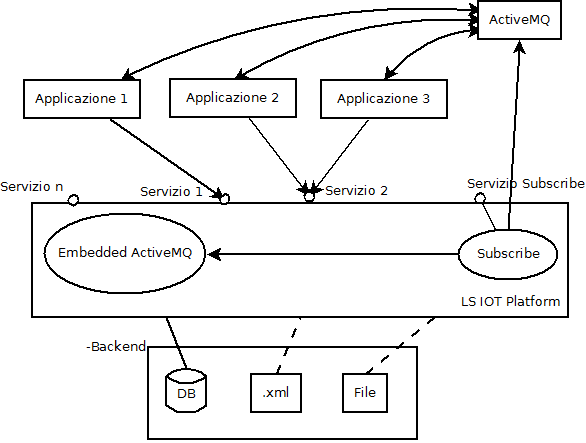
\includegraphics[width=0.9\textwidth]{images/architettura_piattaforma.png}
\end{frame}

\begin{frame}
\frametitle{Pagina catalogo Smart Object}
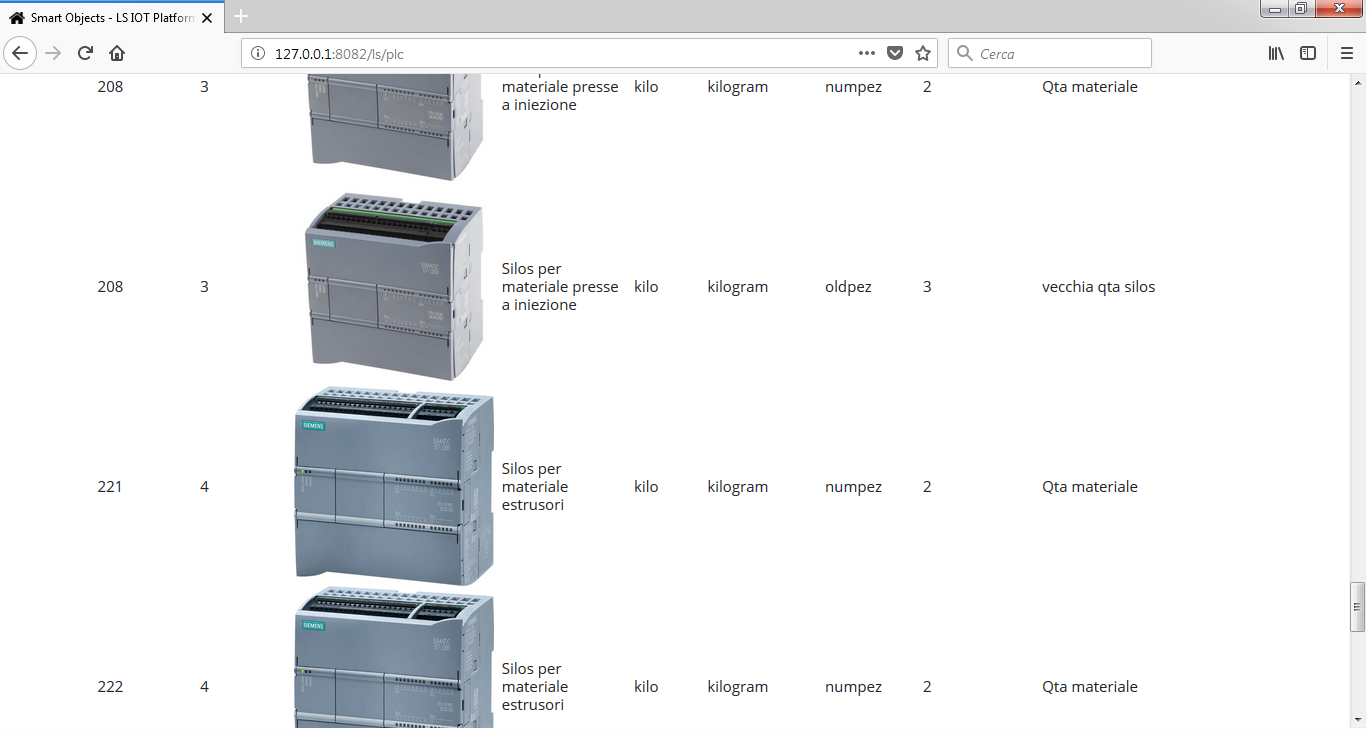
\includegraphics[width=1\textwidth]{images/SmartObjectsPlatform.png}
\end{frame}

\begin{frame}
\frametitle{Esempio valori di ritorno di un servizio}
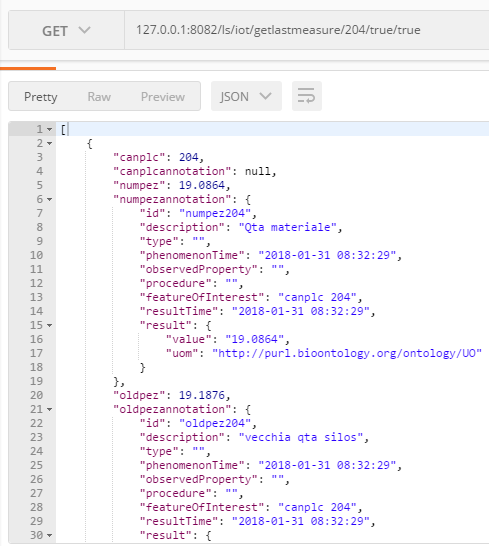
\includegraphics[width=0.6\textwidth]{images/Postman1.png}
\end{frame}

\begin{frame}
\frametitle{Subscribe Rule di una applicazione}
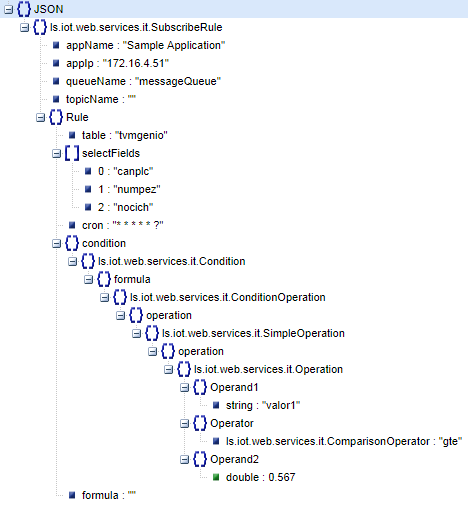
\includegraphics[width=0.6\textwidth]{images/subscribe-json-1.png}
\end{frame}

\begin{frame}
\frametitle{Pagina web per il grafico del monitoraggio}
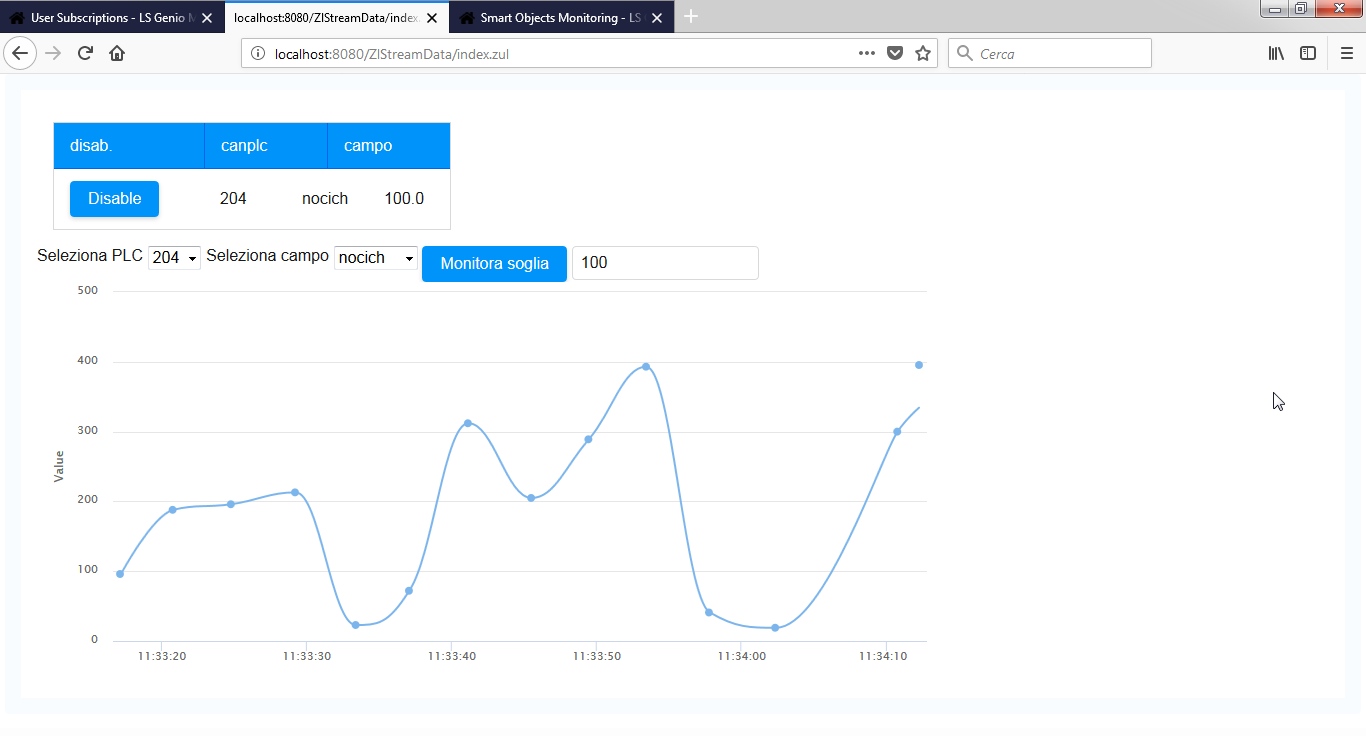
\includegraphics[width=1\textwidth]{images/grafico-zk.png}
\end{frame}

\begin{frame}
\frametitle{Codice Job Flink}
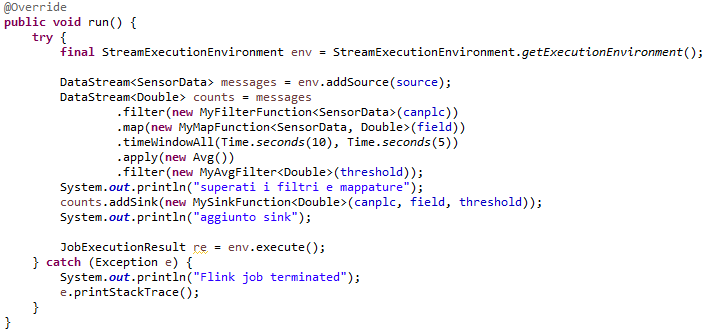
\includegraphics[width=1\textwidth]{images/flink-job.png}
\end{frame}

\begin{frame}
	\frametitle{Conclusioni}
	Questo progetto ha mostrato quanta innovazione e benefici porti alle aziende implementare le novità introdotte dall’Industria 4.0, tra le quali i Big Data rappresentano la componente principale.
\end{frame}

%-------------------------inizio client-----------------------------
\end{document}